\clearpage
\subsubsection{Gate-Treiber}
\label{subsubsec:Gate-Treiber}

%Nebst dem TMC4671, welcher für die Ansteuerung benötigt wird, braucht es für die Magnetisierung der Spulen des BLDC-Motors eine Schaltlogik. Dabei Handelt es sich um den TMC6200. Dieser ist eine umfangreiche Ergänzung zum TMC4671. Auf den TMC6200 und weitere benötigte Komponenten wird im folgenden eingegangen.
%\subsubsection{Problem}\label{subsubsec:Problem_TMC6200}

Der Motor wird über eine H-Brücke gesteuert. Dies bedingt pro Spule zwei MOSFET's, um diese entsprechend magnetisieren zu können. Um einen MOSFET in einen leitenden Zustand zu bringen, muss das Gate des MOSFET's mit einer elektrischen Ladung gefüllt werden. Während diesem Vorgang hat am Gate ein kapazitives Verhalten, was bedeutet, dass bei jedem Schaltvorgang Ströme fliessen. Damit die Umschaltverluste und daraus folgende Abwärme verhindert werden kann, ist es vorteilhaft die Gates so schnell wie möglich laden und entladen zu können. Da kommt der Gate-Treiber ins Spiel. Dieser ladet und entladet das Gate schnell genug und stellt die dazu benötigte Energie für das Gate zur Verfügung.

\paragraph{Schaltungsaufbau}\mbox{}

Damit ein komplizierter Aufbau vermieden werden kann und einige Zusatzfunktionen wie Strommessung, Messverstärkung etc. angeboten werden können, wurde während des Entwicklungsprozesses ein Gate-Treiber von Trinamic ausgewählt. Das entsprechende Bauteil ist der TMC6200. Das Blockdiagramm und eine Beispielschaltung befinden sich im Anhang Kapitel \ref{Appendix:TMC6200} Abbildung \ref{fig:Schaltung_TMC6200} und Abbildung \ref{fig:Blockdiagramm_TMC6200}. Das Blockdiagramm zeigt, dass der TMC6200 aus einer Treiber-Logik für den Motor, einem SPI-/Pinsettings-Interface, einer Diagnosenlogik, Strommessschaltung und diversen unterstützenden Schaltungen wie Spannungsversogrung besteht.

\begin{figure}[h!]
	\centering
	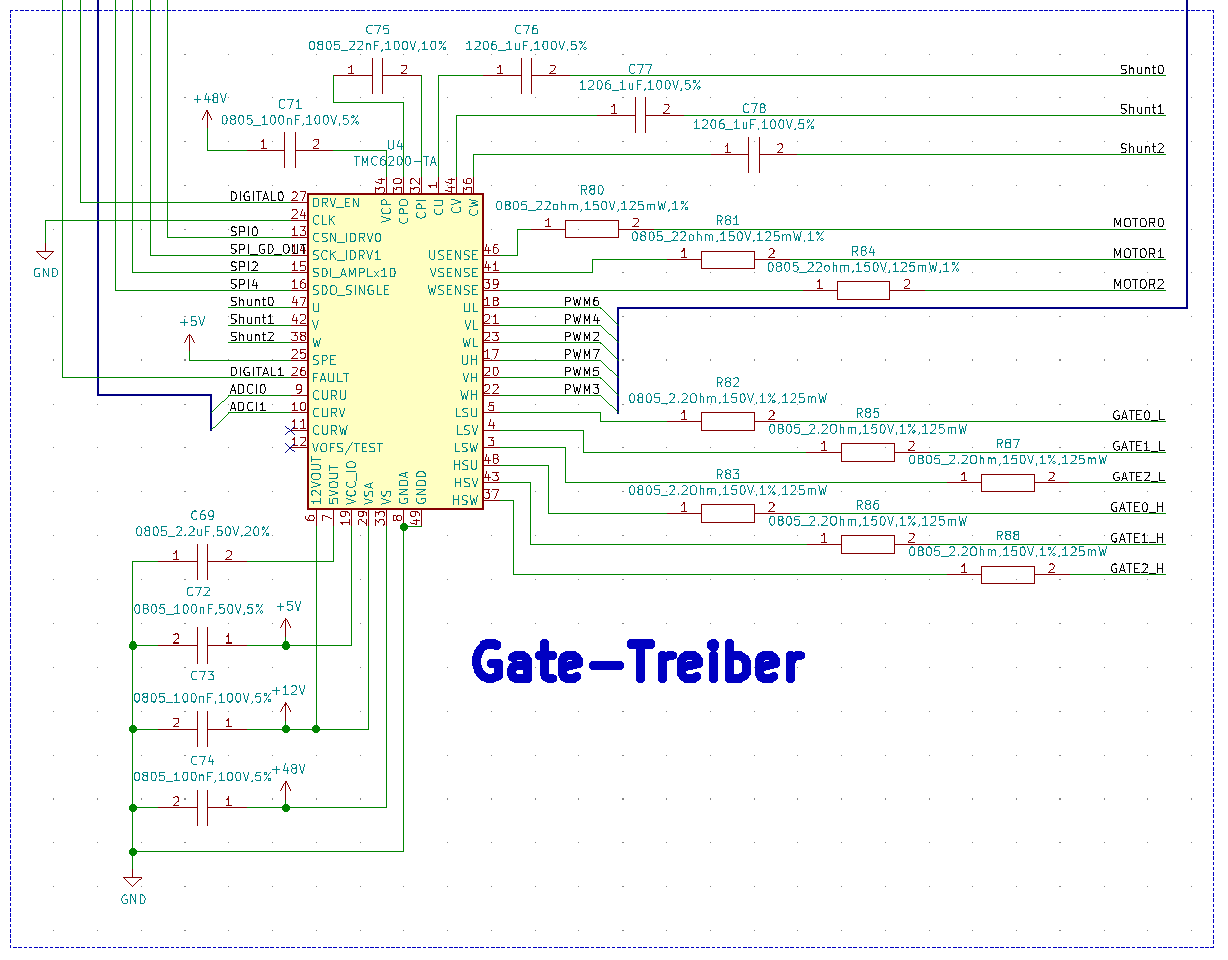
\includegraphics[width=0.8\textwidth]{graphics/Schema_Gate_Treiber}
	\caption{Schema Gate-Treiber.}
	\label{fig:Schema_Gate_Treiber}
\end{figure}
\todo{Kondensatoren/Widerstände im Text erwähnen}
%\begin{figure}[h!]
%	\centering
%	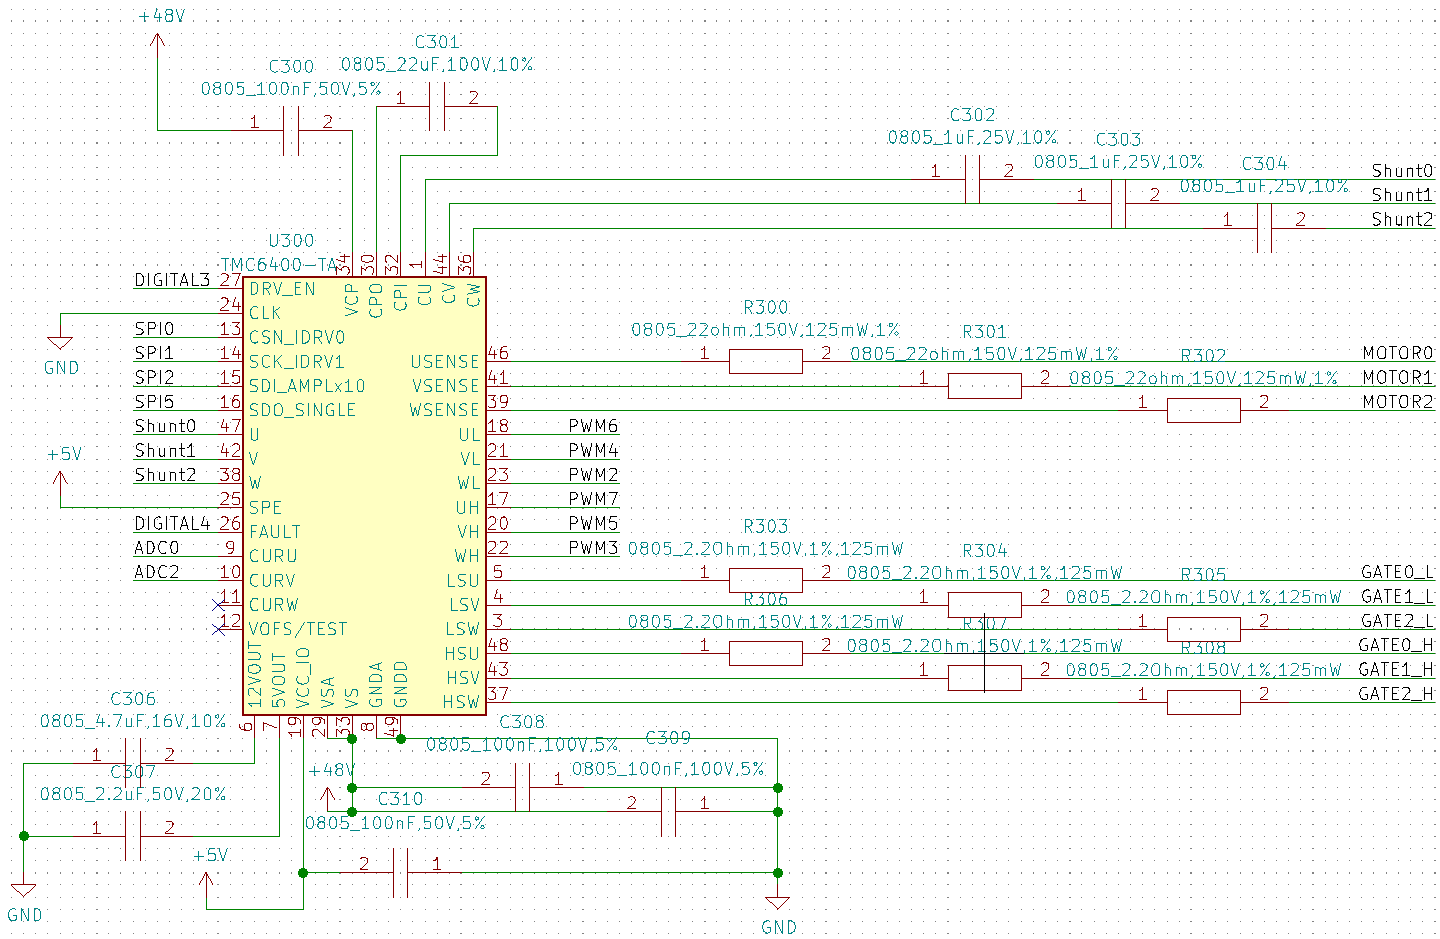
\includegraphics[width=0.8\textwidth]{graphics/TMC6200_Schema.png}
%	\caption{Teilschema Ansteuerung Motor. Hier Gate-Treiber-IC TMC6200.}
%	\label{fig:Schema_TMC6200}
%\end{figure}
%\begin{figure}[h!]
%	\centering
%	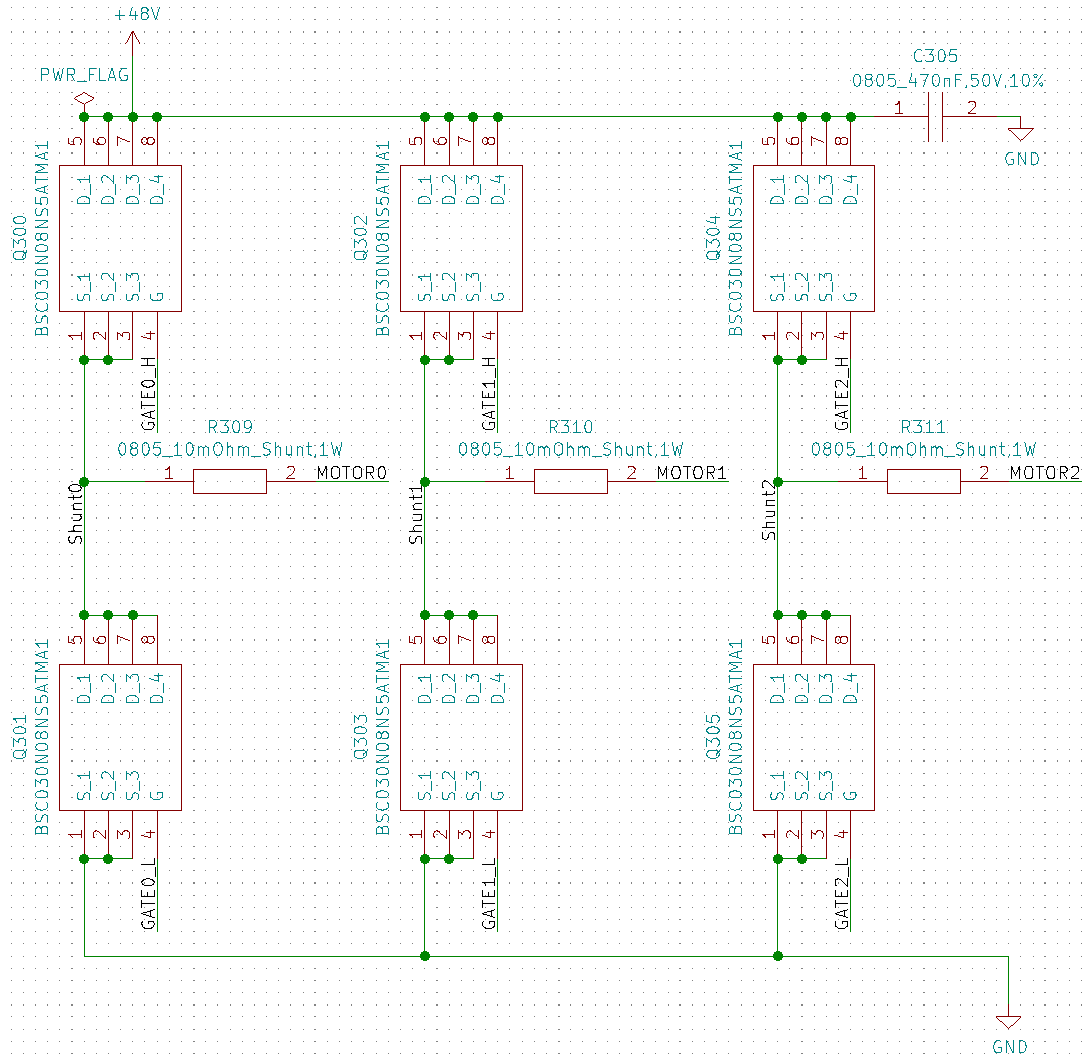
\includegraphics[width=0.6\textwidth]{graphics/H_Bruecke_Schema.png}
%	\caption{Teilschema Ansteuerung Motor. Hier H-Brücke.}
%	\label{fig:Schema_TMC6200}
%\end{figure}

\newpage
\subparagraph{Shunt-Widerstände $\mathrm{\mathbf{R_{Sense}}}$}
Die Shunt-Widerstände ermöglichen einen geschlossenen Loop für die Stromsteuerung, so wie es für eine feldorientierte Steuerung (FOC) benötigt wird. Dazu wird solch ein Shunt in Serie mit der Spule des BLDC-Motors geschaltet. Durch den fliessenden Strom liegt eine Spannung über dem Shunt, welche dann vom TMC6200 verstärkt wird und aufbereitet an den Kontroll-Chip TMC4671 ausgegeben wird. Die Verstärkung sowie Offset auf das Signal sind programmierbar.

Die Dimensionierung der Widerstände und die darauf folgende Programmierung des TMC6200 sind schon von Trinamic ermittelt worden. Es wird empfohlen, die Widerstände nach dem Maximalstrom des Motors auszuwählen. Im Falle des AKM22h sind dies 5A. Darüber hinaus wird empfohlen, eine Überdimensionierung von 25-50\% vorzunehmen. Aus Qualitätsgründen wird jedoch von 10A ausgegangen, was die Zuverlässigkeit und Lebensdauer erhöhen soll, zudem wird so die Verlustleistung des Shunts kleiner gehalten als bei einer Grösse ober-/unterhalb. Eine von Trinamic erstellte Tabelle (siehe Anhang \ref{Appendix:TMC6200} Tabelle \ref{fig:Tabelle_Shunts}) ergibt folgende Grösse für die Shunt-Widerstände: \cite[S.31]{trinamic_tmc6200_datasheet_2013}

\begin{tabular}{lll}
$\mathbf{R_{Sense}}$ =  \textbf{10m\textOmega}\\
\textbf{Verstärkungsfaktor}= \textbf{10x}   
\end{tabular}

\paragraph{Gate Vorwiderstände $\mathrm{\mathbf{R_{Gate}}}$}

Da das Gate ein kapazitives Verhalten zeigt, ist der Strom, welcher zu Beginn ins Gate fliesst, sehr hoch. Der Gate-Vorwiderstand begrenzt diesen, um das Gate und den Pin des TMC6200 vor Überströmen zu schützen.

Die Dimensionierung der Gate-Widerständen sollte grundsätzlich an die MOSFET Gate-Drain- Ladung (Miller charge) angelehnt werden, um an angemessene Anstiegszeiten während des Schaltens zu erreichen. Auch in diesem Falle wurden von Trinamic schon einige Parameter ermittelt und im Anhang \ref{Appendix:TMC6200} in Tabelle \ref{fig:Tabelle_Gatewiderstaende} dargestellt. Die Gate-Ladung des ausgewählten MOSFET's beträgt 61nC. Mit dem programmierbaren Register DRV\_STRENGTH wird der Strom ins Gate angepasst. \cite[S.13]{trinamic_tmc6200_datasheet_2013}

\begin{tabular}{lll}
$\mathrm{\mathbf{R_{Gate}}}$ & \textbf{=} & $\mathrm{\mathbf{R_{Gate}\leq2.5\Omega}}$ \\
\textbf{DRV\_STRENGTH} & \textbf{=} & \textbf{1 bis 3}
\end{tabular}

\paragraph{Schutzwiderstände Messeingang $\mathrm{\mathbf{R_{Protect}}}$}

Wird von einem High-Zustand in einen Low-Zustand gewechselt, kann aufgrund von Induktivitäten der Shunts oder deren Verbindungen die Spannung unterschiessen. Der Schutzwiderstand schützt den Messeingang des TMC6200 vor diesem Effekt.

Die Dimensionierung dieses Widerstands wird im Datenblatt mit einem Widerstandswert zwischen 10\textOmega\ und 22\textOmega\ angegeben.\cite[S.10]{trinamic_tmc6200_datasheet_2013}

\begin{tabular}{lll}
$\mathrm{\mathbf{R_{P}}}$ & \textbf{=} & \textbf{10\textOmega\ bis 22\textOmega}\\
\end{tabular}

\paragraph{Bootstrap Kondensatoren $\mathrm{\mathbf{C_{Bootstrap}}}$}

Die Bootstrap-Kondensator werden benutzt, wenn eine Änderung des Potentials innert kurzer Zeit benötigt wird.

Die Dimensionierung dieses Widerstands wird im Datenblatt mit einem Kapazitätswert zwischen 470nF und 1\textmugreek F angegeben, bei einer Nennspannung von 16V oder 25V. Weiter gilt gemäss Datenblatt, dass bei MOSFET's mit einem $\mathrm{Q_G \geq 40nC}$ die Gatekapazität 1\textmugreek F sein soll. Da die Kapazität 61nF beträgt, ist dies der Fall.\cite[S.10]{trinamic_tmc6200_datasheet_2013}

\begin{tabular}{lll}
$\mathrm{\mathbf{C_{Bootstrap}}}$ & \textbf{=} & \textbf{1\textmugreek F (25V)}\\
\end{tabular}